%!TEX root = da-screen.tex

\chapter{Introduction and Preliminaries}

\section{Scope}

This course focuses on the \emph{theoretical foundations of distributed systems}. Our approach is similar to typical courses on models of computation, computational complexity, and design and analysis of algorithms. The main difference is in the models of computation that we study: instead of traditional models, such as finite state machines, Turing machines, RAM machines, or Boolean circuits, our model of choice is a \emph{distributed system}.

\subsection{Distributed Systems as a Model of Computation}\label{ssec:prelim-model}

A distributed system consists of multiple machines that are connected to each other through communication links. We usually view a distributed system as a (simple, undirected) graph $G = (V,E)$: each node $v \in V$ represents a machine and an edge $\{u,v\} \in E$ represents a communication link between machines $u$ and~$v$.

To understand the key difference between distributed systems and more familiar models of computation, let us consider an illustrative example: the problem of finding a maximal independent set.

An \emph{independent set} for a graph $G = (V,E)$ is a set $I \subseteq V$ such that for each edge $\{u,v\} \in E$ at most one of $u$ and $v$ is in $I$. An independent set $I$ is \emph{maximal} if it cannot be extended, i.e., it is not a proper subset of another independent set.
\begin{center}
    \includegraphics[page=\PIndependentSet]{figs.pdf}
\end{center}

Now given any model of computation $X$ we can pose the familiar question:
\begin{itemize}
    \item \emph{Computability:} is it \emph{possible} to find a maximal independent set in model $X$?
    \item \emph{Computational complexity:} can we find a maximal independent set \emph{efficiently} in model $X$?
\end{itemize}
We are familiar with such questions in the context of Turing machines, but it is not immediately obvious what these questions mean in the context of distributed systems. The following informal comparison illustrates the key differences.
\begin{description}
    \item[Input.] The input is a graph~$G$.
    \begin{descriptionb}
        \item[Turing machines:] We assume that the structure of $G$ is encoded as a string and given to the Turing machine on the input tape.
        \item[Distributed systems:] We assume that the structure of the input graph $G$ is the same as the structure of the distributed system. Initially, each machine $v \in V$ only knows some local information related to $v$ (for example, the degree of $v$ and the unique identifier of $v$). To acquire more information about $G$, the nodes need to exchange messages.
    \end{descriptionb}
    \item[Output.] The output is an independent set $I \subseteq V$.
    \begin{descriptionb}
        \item[Turing machines:] We require that the machine prints an encoding of $I$ on the output tape.
        \item[Distributed systems:] We require that each node $v \in V$ produces one bit of output: if $v \in I$, node $v$ has to output $1$, and if $v \notin I$, node $v$ has to output $0$.
    \end{descriptionb}
    \item[Algorithm.] We say that an algorithm solves the problem if it produces a valid output for any valid input.
    \begin{descriptionb}
        \item[Turing machines:] The algorithm designer chooses the state transitions of the Turing machine.
        \item[Distributed systems:] The algorithm designer writes one program. The same program is installed in each $v \in V$.
    \end{descriptionb}
    \item[Complexity measures.] There are many possible complexity measures, but perhaps the most commonly used is the time complexity.
    \begin{descriptionb}
        \item[Turing machines:] Time = number of elementary steps. In each time unit, (1)~the machine moves the tape heads, (2)~performs a state transition that depends on the contents of the tapes, and (3)~possibly halts.
        \item[Distributed systems:] Time = number of synchronous communication rounds. In each time unit, all machines in parallel (1)~exchange messages with their neighbours, (2)~perform state transitions that depend on the messages that they received, and (3)~possibly halt.
    \end{descriptionb}
\end{description}
To oversimplify a bit, distributed computation is not really about \emph{computation}\mydash it is all about \emph{communication}. Throughout this course, we will see striking examples of the implications of this change of perspective.


\subsection{Outside the Scope}

The term ``distributed computing'' is overloaded, and it means very different things to different people.

For the general public, distributed computing often refers to large-scale high-performance computing in a computer network; this includes scientific computing on grids and clusters, and volunteer computing projects such as SETI@Home and Folding@Home. However, this is \emph{not} the definition that we use, and our course is in no way related to large-scale number crunching.

In general, our focus is on theory, not practice. For our purposes, a communication network is an idealised abstraction. We are not interested in any implementation details or engineering aspects. For example, the following topics are \emph{not} covered on this course: physical properties of wired or wireless media, modulation techniques, communication protocols, standards, software architectures, programming languages, software libraries, privacy, and security.

Within the field of the theory of distributed computing, there are also numerous topics that we are not going to cover. We will conclude this course with a brief overview of other research areas within the field in Section~\ref{sec:other-stuff}.


\chapter{Ramsey Theory}

\section{Introduction}

As a running example in this chapter, we will use the following task: find a $3$-colouring of a directed cycle in the model of unique identifiers.

In a \emph{directed cycle}, we assume that we are given a graph $G = (V,E)$ that is an orientation of a cycle graph. In particular, we assume that each node $v \in V$ has
\[
    \outdegree_G(v) = \indegree_G(v) = 1,
\]
that is, there is precisely one incoming edge and one outgoing edge. Without loss of generality, we will assume that the incoming edge is connected to port number 1 and the outgoing edge is connected to port number 2 in each node \mydash if this was not the case, each node could renumber its ports locally. See Figure~\ref{fig:directed-cycle} for an illustration.

\begin{figure}
    \centering
    \includegraphics[page=\PDirectedCycle]{figs.pdf}
    \caption{A directed cycle with unique identifiers.}\label{fig:directed-cycle}
\end{figure}

Clearly, directed cycles are a special case of directed pseudoforests, and we already know how to find a $3$-colouring of a directed pseudoforest in the model of unique identifiers. Indeed, there are several possible strategies.
\begin{itemize}
    \item The greedy algorithm is simple but slow; in the case of directed cycles, it requires $\Omega(n)$ rounds in the worst case.
    \item Algorithm $\algo{DPBit}$ is much faster\mydash as we saw in Exercise~\ref{ex:logstar}, algorithm $\algo{DPBit}$ finds a $6$-colouring in $O(\log^* n)$ rounds, and we can then use the greedy algorithm to reduce the number of colours from $6$ to $3$ in constant time.
    \item Algorithm $\algo{DPBit}$ is in no way unique, and there are many alternative strategies that we can use to $3$-colour a directed pseudoforest. Exercises \ref{ex:dpbit-base} and \ref{ex:dpset} explore some possible ideas.
\end{itemize}
Moreover, directed cycles are a simple special case of directed pseudoforests, and whenever we have an algorithm that finds a $3$-colouring in any directed pseudoforest, we can construct a slightly faster algorithm that finds a $3$-colouring in directed cycles\mydash for example, we can easily speed up algorithm $\algo{DPGreedy}$ by a factor of two in directed cycles, as the construction of intermediate colouring $s$ becomes unnecessary.

However, no matter what combination of algorithm ideas we use, it appears that the worst-case running time of the algorithm is always $\Omega(\log^* n)$. That is, the running time \emph{slightly} increases as the number of nodes $n$ increases.

In this chapter we will prove that this is indeed necessary. We show that there is no $O(1)$-time algorithm that $3$-colours any directed cycle in the model of unique identifiers. Our proof uses Ramsey's theorem, which is a fundamental result in combinatorics.


\section{Ramsey's Theorem}

Let $Y$ be a finite set. We say that $X$ is a \emph{$k$-subset} of $Y$ if $X \subseteq Y$ and $|X| = k$. We use the notation
\[
    Y^{(k)} = \{ X \subseteq Y : |X| = k \}
\]
for the collection of all $k$-subsets of $Y$.


\subsection{Monochromatic Subsets}

A \emph{$c$-labelling} of $Y^{(k)}$ is an arbitrary function
\[
    f \colon Y^{(k)} \to \{1,2,\dotsc,c\}.
\]
Fix some $Y$, $k$, $c$, and $f$, where $f$ is a $c$-labelling of $Y^{(k)}$. We say that
\begin{enumerate}
    \item $X \subseteq Y$ is \emph{monochromatic in $f$} if $f(A) = f(B)$ for all $A, B \in X^{(k)}$,
    \item $X \subseteq Y$ is \emph{almost monochromatic in $f$} if $f(A) = f(B)$ for all $A, B \in X^{(k)}$ with $\min(A) = \min(B)$.
\end{enumerate}
See Figure~\ref{fig:monochromatic} for examples. Monochromatic subsets are a central concept in Ramsey theory, while almost monochromatic subsets are a technical definition that we will use in the proof.

\begin{figure}
    \centering
    \begin{tabular}{c@{\hspace{5ex}}c}
        \toprule
        \multicolumn{2}{@{}c@{}}{$f \colon Y^{(2)} \to \{1,2,3\}$} \\
        \midrule
        $\{1,2\} \mapsto 1$ & $\{2,4\} \mapsto 1$ \\ 
        $\{1,3\} \mapsto 1$ & $\{2,5\} \mapsto 2$ \\
        $\{1,4\} \mapsto 2$ & $\{3,4\} \mapsto 3$ \\
        $\{1,5\} \mapsto 1$ & $\{3,5\} \mapsto 3$ \\
        $\{2,3\} \mapsto 2$ & $\{4,5\} \mapsto 3$ \\
        \bottomrule
    \end{tabular}
    \caption{In this example, $Y = \{1,2,3,4,5\}$. Function $f$ is a $3$-labelling of $Y^{(2)}$. Set $\{1,2,3,5\}$ is almost monochromatic but not monochromatic in $f$. Set $\{3,4,5\}$ is both almost monochromatic and monochromatic in $f$.}\label{fig:monochromatic}
\end{figure}


\subsection{Ramsey Numbers}

For all positive integers $c$, $n$, and $k$, we define the numbers $R_c(n;k)$ and $\bar{R}_c(n;k)$ as follows.
\begin{enumerate}
    \item $R_c(n;k)$ is the smallest natural number $N$ such that the following holds: for any set $Y$ with at least $N$ elements, and for any $c$-labelling $f$ of $Y^{(k)}$, there is an $n$-subset of $Y$ that is monochromatic in $f$. If no such $N$ exists, $R_c(n;k) = \infty$.
    \item $\bar{R}_c(n;k)$ is the smallest natural number $N$ such that the following holds: for any set $Y$ with at least $N$ elements, and for any $c$-labelling $f$ of $Y^{(k)}$, there is an $n$-subset of $Y$ that is almost monochromatic in $f$. If no such $N$ exists, $\bar{R}_c(n;k) = \infty$.
\end{enumerate}
Numbers $R_c(n;k)$ are called \emph{Ramsey numbers}, and Ramsey's theorem shows that they are always finite.

\begin{theorem}[Ramsey's theorem]\label{thm:ramsey}
    Numbers $R_c(n;k)$ are finite for all positive integers $c$, $n$, and $k$.
\end{theorem}

We will prove Theorem~\ref{thm:ramsey} in Section~\ref{ssec:ramsey-proof}; let us first have a look at an application.


\subsection{An Application}

In the case of $k = 2$, Ramsey's theorem can be used to derive various graph-theoretic results. As a simple application, we can use Ramsey's theorem to prove that sufficiently large graphs necessarily contain large cliques or large independent sets.

Let $G = (V,E)$ be a graph. Recall that an \emph{independent set} is a subset $X \subseteq V$ such that $\{u,v\} \notin E$ for all $\{u, v\} \in X^{(2)}$. A complementary concept is a \emph{clique}: it is a subset $X \subseteq V$ such that $\{u,v\} \in E$ for all $\{u, v\} \in X^{(2)}$.

\begin{lemma}
    For any natural number $n$ there is a natural number $N$ such that the following holds:
    if $G = (V,E)$ is a graph with at least $N$ nodes,
    then $G$ contains a clique with $n$ nodes or an independent set with $n$ nodes.
\end{lemma}
\begin{proof}
    Choose an integer $N \ge R_2(n;2)$; by Theorem~\ref{thm:ramsey}, such an $N$ exists.
    
    Now if $G = (V,E)$ is any graph with at least $N$ nodes, we can define a $2$-labelling $f$ of $V^{(2)}$ as follows:
    \[
        f(\{u,v\}) = \begin{cases}
            1 & \text{if } \{u,v\} \in E, \\
            2 & \text{if } \{u,v\} \notin E.
        \end{cases}
    \]
    By the definition of Ramsey numbers, if $|V| \ge N$, there is an $n$-subset $X \subseteq V$ that is monochromatic in $f$.
    If $X \subseteq V$ is monochromatic, we have one of the following cases:
    \begin{enumerate}
        \item we have $f(\{u,v\}) = 1$ for all $\{u,v\} \in X^{(2)}$; therefore $X$ is a clique,
        \item we have $f(\{u,v\}) = 2$ for all $\{u,v\} \in X^{(2)}$; therefore $X$ is an independent set. \qedhere
    \end{enumerate}
\end{proof}


\subsection{Proof}\label{ssec:ramsey-proof}

Let us now prove Theorem~\ref{thm:ramsey}. Throughout this section, let $c$ be fixed. We will show that $R_c(n;k)$ is finite for all $n$ and $k$. The proof outline is as follows:
\begin{enumerate}
    \item Lemma~\ref{lem:pigeonhole}: $R_c(n;1)$ is finite for all $n$.
    \item Corollary~\ref{cor:RtoR}: if $R_c(n;k-1)$ is finite for all $n$, then $R_c(n;k)$ is finite for all $n$.
    
        Here we will use the following auxiliary results:
        \begin{enumerate}[label=(\roman*)]
            \item Lemma~\ref{lem:RtoG}\mydash if $R_c(n;k-1)$ is finite for all $n$, then $\bar{R}_c(n;k)$ is finite for all $n$.
            \item Lemma~\ref{lem:GtoR}\mydash if $\bar{R}_c(n;k)$ is finite for all $n$, then $R_c(n;k)$ is finite for all $n$.
        \end{enumerate}
    \item Now by induction on $k$, it follows that $R_c(n;k)$ is finite for all $n$ and $k$.
\end{enumerate}

The base case of $k = 1$ is, in essence, equal to the familiar pigeonhole principle.

\begin{lemma}\label{lem:pigeonhole}
    Ramsey number $R_c(n;1)$ is finite for all $n$.
\end{lemma}
\begin{proof}
    Let $N = c(n-1)+1$. We can use the pigeonhole principle to show that $R_c(n;1) \le N$.
    
    Let $Y$ be a set with at least $N$ elements, and let $f$ be a $c$-labelling of $Y^{(1)}$.
    In essence, we have $c$ boxes, labelled with $\{1,2,\dotsc,c\}$, and function $f$ places each element of $Y$ into one of these boxes.
    As there are $N$ elements, there is a box that contains at least
    \[
        \lceil N/c \rceil = n
    \]
    elements. These elements form a monochromatic subset.
\end{proof}

Let us now study the case of $k > 1$. We begin with a technical lemma.

\begin{lemma}\label{lem:RtoGpart}
    Let $n$ and $k$ be integers, $n > k > 1$.
    If $M = \bar{R}_c(n-1;k)$ and $R_c(M;k-1)$ are finite, then $\bar{R}_c(n;k)$ is finite.
\end{lemma}
\begin{proof}
    Define
    \[
        N = 1 + R_c(M;k-1).
    \]
    We will prove that $\bar{R}_c(n;k) \le N$.
    
    Let $Y$ be a set with $N$ elements; w.l.o.g., we can assume that $Y = \{1,2,\dotsc,N\}$. Let $f$ be any $c$-labelling of $Y^{(k)}$. We need to show that there is an almost monochromatic $n$-subset $W \subseteq Y$.
    
    To this end, let $Y_2 = \{2,3,\dotsc,N\}$, and define a $c$-labelling $f_2$ of $Y_2^{(k-1)}$ as follows; see Figure~\ref{fig:RtoGpart} for an illustration:
    \[
        f_2(A) = f(\{1\} \cup A) \ \text{ for each } A \in Y_2^{(k-1)}.
    \]
    Now $f_2$ is a $c$-labelling of $Y_2^{(k-1)}$, and $Y_2$ contains
    \[
        N - 1 = R_c(M;k-\nobreak 1)
    \]    
    elements. Hence, by the definition of Ramsey numbers, there is an $M$-subset $X_2 \subseteq Y_2$ that is monochromatic in $f_2$.

\begin{figure}
    \centering
    \includegraphics[page=\PRtoGPart]{figs.pdf}
    \caption{The proof of Lemma~\ref{lem:RtoGpart}, for the case of $c = 2$, $k = 3$, and $n = 5$, assuming completely fictional values $M = 5$ and $N = 7$.}\label{fig:RtoGpart}
\end{figure}
    
    Function $f$ is a $c$-labelling of $Y^{(k)}$, and $X_2 \subseteq Y$. Hence by restriction $f$ defines a $c$-labelling of $X_2^{(k)}$. Set $X_2$ contains $M = \bar{R}_c(n-\nobreak 1;k)$ elements. Therefore there is an $(n-\nobreak 1)$-subset $W_2 \subseteq X_2$ that is almost monochromatic in $f$.
    
    To conclude the proof, let $W = \{1\} \cup W_2$. By construction, $W$ contains $n$ elements. Moreover, $W$ is almost monochromatic in $f$. To see this, assume that $A,B \subseteq W$ are $k$-subsets such that $\min(A) = \min(B)$. We need to show that $f(A) = f(B)$. There are two cases:
    \begin{enumerate}
        \item We have $\min(A) = \min(B) = 1$. Let $A_2 = A \setminus \{1\}$ and $B_2 = B \setminus \{1\}$. Now $A_2$ and $B_2$ are $(k-1)$-subsets of $X_2$. Set $X_2$ was monochromatic in $f_2$, and hence $f(A) = f_2(A_2) = f_2(B_2) = f(B)$.
        \item Otherwise $1 \notin A$ and $1 \notin B$. Now $A$ and $B$ are $k$-subsets of $W_2$. Set $W_2$ was almost monochromatic in $f$, and we have $\min(A) = \min(B)$, which implies $f(A) = f(B)$. \qedhere
    \end{enumerate}
\end{proof}

\begin{lemma}\label{lem:RtoG}
    Let $k > 1$ be an integer.
    If $R_c(n;k-1)$ is finite for all $n$, then $\bar{R}_c(n;k)$ is finite for all $n$.
\end{lemma}
\begin{proof}
    The proof is by induction on $n$.
    
    The base case of $n \le k$ is trivial: a set with $n$ elements has at most one subset with $k$ elements, and hence it is almost monochromatic and monochromatic.
    
    Now let $n > k$. Inductively assume that $\bar{R}_c(n-1;k)$ is finite. Recall that in the statement of this lemma, we assumed that $R_c(M;k-1)$ is finite for any $M$; in particular, it is finite for $M = \bar{R}_c(n-1;k)$. Hence we can apply Lemma~\ref{lem:RtoGpart}, which implies that $\bar{R}_c(n;k)$ is finite.
\end{proof}

\begin{lemma}\label{lem:GtoR}
    Let $k > 1$ be an integer.
    If $\bar{R}_c(n;k)$ is finite for all $n$, then $R_c(n;k)$ is finite for all $n$.
\end{lemma}
\begin{proof}
    Let $M = R_c(n;1)$. By Lemma~\ref{lem:pigeonhole}, $M$ is finite. By assumption, $\bar{R}_c(M;k)$ is also finite. We will show that
    \[
        R_c(n;k) \le \bar{R}_c(M;k).
    \]
    
    Let $Y$ be a set with $N = \bar{R}_c(M;k)$ elements, and let $f$ be any $c$-labelling of $Y^{(k)}$. We need to show that there is a monochromatic $n$-subset $W \subseteq Y$.
    
    By definition, there is an almost monochromatic $M$-subset $X \subseteq Y$. Hence we can define a $c$-labelling $g$ of $X^{(1)}$ such that
    \[
        g( \{ \min(A) \} ) = f(A)
    \]
    for each $k$-subset $A \subseteq X$; see Figure~\ref{fig:GtoR}. As $X$ is a subset with $M = R_c(n;1)$ elements, we can find an $n$-subset $W \subseteq X$ that is monochromatic in $g$.

\begin{figure}
    \centering
    \begin{tabular}{c@{\hspace{5ex}}c}
        \toprule
        $f$ & $g$ \\
        \midrule
        $\{1,2\} \mapsto 1$ & $\{1\} \mapsto 1$ \\ 
        $\{1,3\} \mapsto 1$ & \\
        $\{1,4\} \mapsto 1$ & \\
        \midrule
        $\{2,3\} \mapsto 3$ & $\{2\} \mapsto 3$ \\
        $\{2,4\} \mapsto 3$ & \\
        \midrule
        $\{3,4\} \mapsto 2$ & $\{3\} \mapsto 2$ \\
        \midrule
                            & $\{4\} \mapsto 1$ \\
        \bottomrule
    \end{tabular}
    \caption{The proof of Lemma~\ref{lem:GtoR}. In this example, $c=3$, $k=2$, and $X = \{1,2,3,4\}$ is almost monochromatic in $f$. We define a $c$-labelling $g$ of $X^{(1)}$ such that $g( \{ \min(A) \} ) = f(A)$ for all $A \in X^{(2)}$. Note that the choice of $g({4})$ is arbitrary.}\label{fig:GtoR}
\end{figure}
    
    Now we claim that $W$ is also monochromatic in $f$. To see this, let $A$ and $B$ be $k$-subsets of $W$. Let $x = \min(A)$ and $y = \min(B)$. We have $x, y \in W$ and
    \[
        f(A) = g(\{x\}) = g(\{y\}) = f(B). \qedhere
    \]
\end{proof}

Lemmas \ref{lem:RtoG} and \ref{lem:GtoR} have the following corollary.

\begin{corollary}\label{cor:RtoR}
    Let $k > 1$ be an integer.
    If $R_c(n;k-1)$ is finite for all $n$, then $R_c(n;k)$ is finite for all $n$.
\end{corollary}

Now Ramsey's theorem follows by induction on $k$: the base case is Lemma~\ref{lem:pigeonhole}, and the inductive step is Corollary~\ref{cor:RtoR}.


\section{Speed Limits}\label{sec:speed-limits}

We will now use Ramsey's theorem to prove that directed cycles cannot be $3$-coloured in constant time.

\begin{theorem}\label{thm:colour-lb}
    Assume that $A$ is a distributed algorithm for the model of unique identifiers. Assume that there is a constant $T \in \NN$ such that $A$ stops in time $T$ in any directed cycle $G = (V,E)$, and outputs a labelling $g\colon V \to \{1,2,3\}$. Then there exists a directed cycle $G$ such that if we execute $A$ on $G$, the output of $A$ is not a proper vertex colouring of~$G$.
\end{theorem}

To prove Theorem~\ref{thm:colour-lb}, let $n = 2T+2$, $k = 2T+1$, and $c = 3$. By Ramsey's theorem, $R_c(n;k)$ is finite. Choose any $N \ge R_c(n;k)$.

We will construct a directed cycle $G = (V,E)$ with $N$ nodes. In our construction, the set of nodes is $V = \{1,2,\dotsc,N\}$. This is also the set of unique identifiers in our cycle; recall that we follow the convention that the unique identifier of a node $v \in V$ is $v$.

With the set of nodes fixed, we proceed to define the set of edges. In essence, we only need to specify in which order the nodes are placed along the cycle.

\subsection{Subsets and Cycles}

For each subset $X \subseteq V$, we define a directed cycle $G_X = (V,E_X)$ as follows; see Figure~\ref{fig:subset-cycle}. Let $\ell = |X|$. Label the nodes by $x_1, x_2, \dotsc, x_N$ such that
\begin{align*}
    X &= \Set{ x_1, x_2, \dotsc, x_{\ell} }, \\
    V \setminus X &= \Set{ x_{\ell+1}, x_{\ell+1}, \dotsc, x_N }, \\
    x_1 &< x_2 < \dotsb < x_{\ell}, \\
    x_{\ell+1} &< x_{\ell+1} < \dotsb < x_N.
\end{align*}
Then choose the edges
\[
    E_X = \Set{ (x_i, x_{i+1}) : 1 \le i < N } \, \cup \, \Set{ (x_N,x_1) }.
\]

\begin{figure}
    \centering
    \includegraphics[page=\PSubsetCycle]{figs.pdf}
    \caption{Construction of $G_X$. Here $N = 6$ and $X = \{2,4\}$.}\label{fig:subset-cycle}
\end{figure}

Informally, $G_X$ is constructed as follows: first take all nodes of $X$, in the order of increasing identifiers, and then take all other nodes, again in the order of increasing identifiers.


\subsection{Labelling}

If $B \subseteq V$ is a $k$-subset, then we define that the \emph{internal node} $i(B)$ is the median of the set $B$. Put otherwise, $i(B)$ is the unique node in $B$ that is not among the $T$ smallest nodes of $B$, nor among the $T$ largest nodes of $B$.

We will use algorithm $A$ to construct a $c$-labelling $f$ of $V^{(k)}$ as follows. For each $k$-subsets $B \subseteq V$, we construct the cycle $G_B$, execute $A$ on $G_B$, and define that $f(B)$ is the output of node $i(B)$ in $G_B$. See Figure~\ref{fig:colour-lb} for an illustration.

\begin{figure}
    \centering
    \includegraphics[page=\PColourLB]{figs.pdf}
    \caption{In this example, $N = 10$ and $T = 2$. Let $B = \Set{1,2,4,5,7}$, $C = \Set{2,4,5,7,9}$, and $X = \Set{1,2,4,5,7,9}$. The label $f(B)$ is defined as follows: we construct $G_B$, execute algorithm $A$, and take the output of the internal node $i(B) = 4$. Similarly, the label $f(C)$ is the output of node $i(C) = 5$ in $G_C$. As the local neighbourhoods are identical, the output of node $4$ in $G_X$ is also $f(B)$, and the output of node $5$ in $G_X$ is also $f(C)$. If $X$ is monochromatic in $f$, we have $f(B) = f(C)$.}\label{fig:colour-lb}
\end{figure}


\subsection{Monochromatic Subsets}

We have constructed a certain $c$-labelling $f$. As $N$ is sufficiently large, there exists an $n$-subset $X \subseteq V$ that is monochromatic in~$f$. Let us label the nodes of $X$ by
\[
    X = \{ x_0, x_1, \dotsc, x_k \},
\]
where $x_0 < x_1 < \dotsb < x_k$. Let
\begin{align*}
    B &= \{ x_0,x_1,\dotsc,x_{k-1} \}, \\
    C &= \{ x_1,x_2,\dotsc,x_k \}.
\end{align*}
See Figure~\ref{fig:colour-lb} for an illustration.

Sets $B$ and $C$ are $k$-subsets of $X$, and their internal nodes are $i(B) = x_{T}$ and $i(C) = x_{T+1}$. As $X$ is monochromatic, we have $f(B) = f(C)$. Therefore we know that the output of $x_{T}$ in $G_B$ equals the output of $x_{T+1}$ in $G_C$.

Moreover, node $x_{T}$ has isomorphic radius-$T$ neighbourhoods in $G_B$ and $G_X$; in both graphs, the radius-$T$ neighbourhood of node $x_{T}$ is a directed path, along which we have the nodes $x_0,x_1,\dotsc,\allowbreak x_{k-1}$ in this order. Hence by Theorem~\ref{thm:local-neighbourhood}, the output of $x_{T}$ in $G_B$ equals the output of $x_{T}$ in $G_X$.

A similar argument shows that the output of $x_{T+1}$ in $G_C$ equals the output of $x_{T+1}$ in $G_X$. In summary, the output of $x_{T}$ in $G_X$ equals $f(B)$, which equals $f(C)$, which equals the output of $x_{T+1}$ in $G_X$.

We have shown that in the directed cycle $G_X$, there are two adjacent nodes, $x_T$ and $x_{T+1}$, that produce the same output. Hence $A$ does not output a proper vertex colouring in $G_X$.


\section{Exercises}

\begin{ex}
    Prove that $R_c(n;1) = c(n-1)+1$.
    
    \hint{The proof of Lemma~\ref{lem:pigeonhole} shows that \[R_c(n;1) \le c(n-1)+1.\] You need to show that \[R_c(n;1) > c(n-\nobreak 1).\]}
\end{ex}

\begin{ex}
    Prove that $R_2(3;2) = 6$.
\end{ex}

\begin{ex}
    Prove that it is not possible to find a proper vertex colouring with at most $100$ colours in any directed cycle in constant time.

    \hint{You can modify the proof of Theorem~\ref{thm:colour-lb}. Alternatively, you can show that if you could find a $100$-colouring in constant time, you could also find a $3$-colouring in constant time.}
\end{ex}

\begin{ex}
    Prove that it is not possible to find a maximal independent set in any directed cycle in constant time.

    \hint{Assume that algorithm $A$ finds an independent set in time $T$ in any directed cycle. Follow the basic idea of the proof of Theorem~\ref{thm:colour-lb}. Choose $n = 2T+3$, $k = 2T+1$, and $c = 2$. Show that you can construct a cycle in which a node and \emph{both} of its neighbours produce the same output. Argue that if the output is a valid independent set, it cannot be a maximal independent set.}
\end{ex}

\begin{ex}
    Prove that it is not possible to find a maximal matching in any directed cycle in constant time.
\end{ex}

\begin{ex}\label{ex:is-apx-lb}
    Prove that it is not possible to find a \Apx{100} of a maximum independent set in any directed cycle in constant time.
    
    \hint{You will need several applications of Ramsey's theorem. First, choose a (very large) space of unique identifiers. Then apply Ramsey's theorem to find a large monochromatic subset, remove the set, and repeat. This way you have partitioned \emph{almost} all identifiers into monochromatic subsets. Each monochromatic subset is used to construct a fragment of the cycle.}
\end{ex}



\chapter{What Next?}

\section{Other Stuff Exists}\label{sec:other-stuff}

Distributed computing is a vast topic. We conclude this course by mentioning perspectives that we have not covered; we also provide pointers to more in-depth information.

\subsection{Models of Computing}

Many models of distributed computing can be seen as extensions of the models that we have studied. The following extensions are familiar from the context of classical computational complexity and Turing machines.
\begin{description}
    \item[Randomised algorithms.] Each node has access to a stream of random bits. A good example is Luby's~\cite{luby86simple} randomised algorithm for finding a maximal independent set\mydash the algorithm uses the random bits for symmetry breaking.
    \item[Nondeterministic algorithms.] It is sufficient that there exists a \emph{proof} that can be verified efficiently in a distributed setting; we do not need to construct the proof. This research direction was introduced by Korman et al.~\cite{korman05proof}.
\end{description}

\subsection{Variants}

There are many variants of the model that we described.
\begin{description}
    \item[Asynchronous systems.] Computers do not necessarily operate in a synchronous manner. In particular, the propagation delays of the messages may vary.
    \item[Message passing vs.\ shared memory.] Our model of computing can be seen as a \emph{message-passing system}: nodes send messages (data packets) to each other. A commonly studied alternative is a system with \emph{shared memory}: each node has a shared register, and the nodes can communicate with each other by reading and writing the shared registers.
\end{description}
The above aspects were irrelevant for our purposes, as we were only interested in the number of communication rounds; for example, asynchronous systems can be ``synchronised'' efficiently~\cite{awerbuch85complexity}. However, if we consider other complexity measures or fault tolerance, such details become important.

Our model of computing is primarily intended to capture the specifics of \emph{wired} networks\mydash communication links can be seen as cables that connect the computers. There are also numerous models that are designed with \emph{wireless} networks in mind. A simple graph is no longer an appropriate model: a single radio transmission can be received by multiple nodes, and multiple simultaneous radio transmissions can interfere with each other. Radio propagation is closely connected with physical distances; hence in the context of wireless networks one often makes assumptions about \emph{physical locations} of the nodes.

\subsection{Complexity Measures}\label{ssec:next-compl-meas}

For us, the main complexity measure has been the number of synchronous communication rounds. Naturally, other possibilities exist.
\begin{description}
    \item[Space.] How many bits of memory do we need per node?
    \item[Number of messages.] How many messages do we need to send in total?
    \item[Message size.] We did not limit the size of a message. However, it is common to assume that the size of each message is $O(\log n)$ bits; how many communication rounds do we need in that case?
\end{description}

\subsection{Fault Tolerance and Dynamics}\label{ssec:next-fault}

Fault tolerance in general is an important topic in any large-scale distributed system. In the theory of distributed computing, fault tolerance has been studied from many different and complementary perspectives, of which we mention three representative examples.
\begin{description}
    \item[Dynamic networks.] Nodes can join and leave; edges can be removed and added. The system is expected to correct the output quickly after each change.
    \item[Byzantine failures.] A fraction of nodes can be malicious and they may try to actively disturb the algorithm. Nevertheless, non-malicious nodes must be able to produce a correct output.
    \item[Self-stabilising systems.] The initial state of each node can be arbitrary\mydash an adversary may have corrupted the memory of each node. Nevertheless, the system must eventually recover and produce a correct output. Note that a self-stabilising system can never stop; all nodes have to keep communicating with each other indefinitely. See Dolev's~\cite{dolev00self-stabilization} textbook for more information.
\end{description}

\subsection{Problems}

In this course we have studied \emph{input/output problems}: we are given an input, we expect the system to do some computation, and eventually the system has to produce a correct output.

We assumed that the input is equal to the structure of the communication graph. This is not the only possibility: in general, one can solve arbitrary input/output problems in a distributed manner.

However, there are also many problems that are \emph{not} input/output problems. In the context of distributed algorithms, there are also problems that are related to \emph{controlling} an autonomous entity. Often we will use the metaphor of robot navigation: the graph is a map of an environment, and we need to control ``robots'' that navigate in the graph\mydash however, instead of a physical robot, we can equally well study a logical entity such as a data packet or a token that is routed throughout a network. Some examples of robot navigation tasks include the following.
\begin{description}
    \item[Graph exploration.] A robot needs to visit all nodes of a graph.
    \item[Rendezvous.] There are two robots who need to meet each other at a single node.
\end{description}

